\documentclass[a4paper, 14pt]{extarticle}
\usepackage[russian]{babel}
\usepackage[T1]{fontenc}
\usepackage{fontspec}
\usepackage{indentfirst}
\usepackage{enumitem}
\usepackage{graphicx}
\usepackage[
  left=20mm,
  right=10mm,
  top=20mm,
  bottom=20mm
]{geometry}
\usepackage{parskip}
\usepackage{titlesec}
\usepackage{xurl}
\usepackage{hyperref}
\usepackage{float}
\usepackage[
  figurename=Рисунок,
  labelsep=endash,
]{caption}
\usepackage[outputdir=build, newfloat]{minted}

\hypersetup{
  colorlinks=true,
  linkcolor=black,
  filecolor=blue,
  urlcolor=blue,
}

\renewcommand*{\labelitemi}{---}
\setmainfont{Times New Roman}
\setmonofont{JetBrains Mono}[
  SizeFeatures={Size=11},
]

\newenvironment{code}{\captionsetup{type=listing}}{}
\SetupFloatingEnvironment{listing}{name=Листинг}

\setminted{
  fontsize=\footnotesize,
}

\setlength{\parskip}{6pt}

\setlength{\parindent}{1cm}
\setlist[itemize]{itemsep=0em,topsep=0em,parsep=0em,partopsep=0em,leftmargin=2.0cm,wide}
\setlist[enumerate]{itemsep=0em,topsep=0em,parsep=0em,partopsep=0em,leftmargin=2.0cm,wide}

\renewcommand{\thesection}{\arabic{section}.}
\renewcommand{\thesubsection}{\thesection\arabic{subsection}.}
\renewcommand{\thesubsubsection}{\thesubsection\arabic{subsubsection}.}

\titleformat{\section}{\normalfont\bfseries}{\thesection}{0.5em}{}
\titleformat{\subsection}{\normalfont\bfseries}{\thesubsection}{0.5em}{}

\titleformat*{\section}{\normalfont\bfseries}
\titleformat*{\subsection}{\normalfont\bfseries}

\linespread{1.5}
\renewcommand{\baselinestretch}{1.5}

\begin{document}

\begin{titlepage}
  \vspace{0pt plus2fill}
  \noindent

  \vspace{0pt plus6fill}
  \begin{center}
    Санкт-Петербургский национальный исследовательский университет
    информационных технологий, механики и оптики

    \vspace{0pt plus3fill}

    Факультет инфокоммуникационных технологий

    Направление подготовки 11.03.02

    \vspace{0pt plus2fill}

    Лабораторная работа №5
  \end{center}

  \vspace{0pt plus6fill}
  \begin{flushright}
    Выполнил: \\
    Швалов Даниил Андреевич

    Группа: К33211

    Проверила: \\
    Марченко Елена Вадимовна
  \end{flushright}

  \vspace{0pt plus5fill}
  \begin{center}
    Санкт-Петербург

    2024
  \end{center}
\end{titlepage}

\section{Введение}

\textbf{Цель работы}: разработать мобильное приложение для подключения к БД
\foreignlanguage{english}{PostgreSQL} с помощью Flutter.

\section{Ход работы}

\subsection*{Создание первого приложения}

С официального сайта Flutter был загружен и установлен Flutter SDK. После
установки в командной строке появилась новая утилита flutter. С ее помощью,
командой <<\foreignlanguage{english}{flutter create my\_app}>> было создано
новое приложение <<\foreignlanguage{english}{my\_app}>>.

Для разработки мобильного приложения был открыт эмулятор iOS (рисунок
\ref{fig:task-1-1}).

\begin{figure}[H]
  \centering
  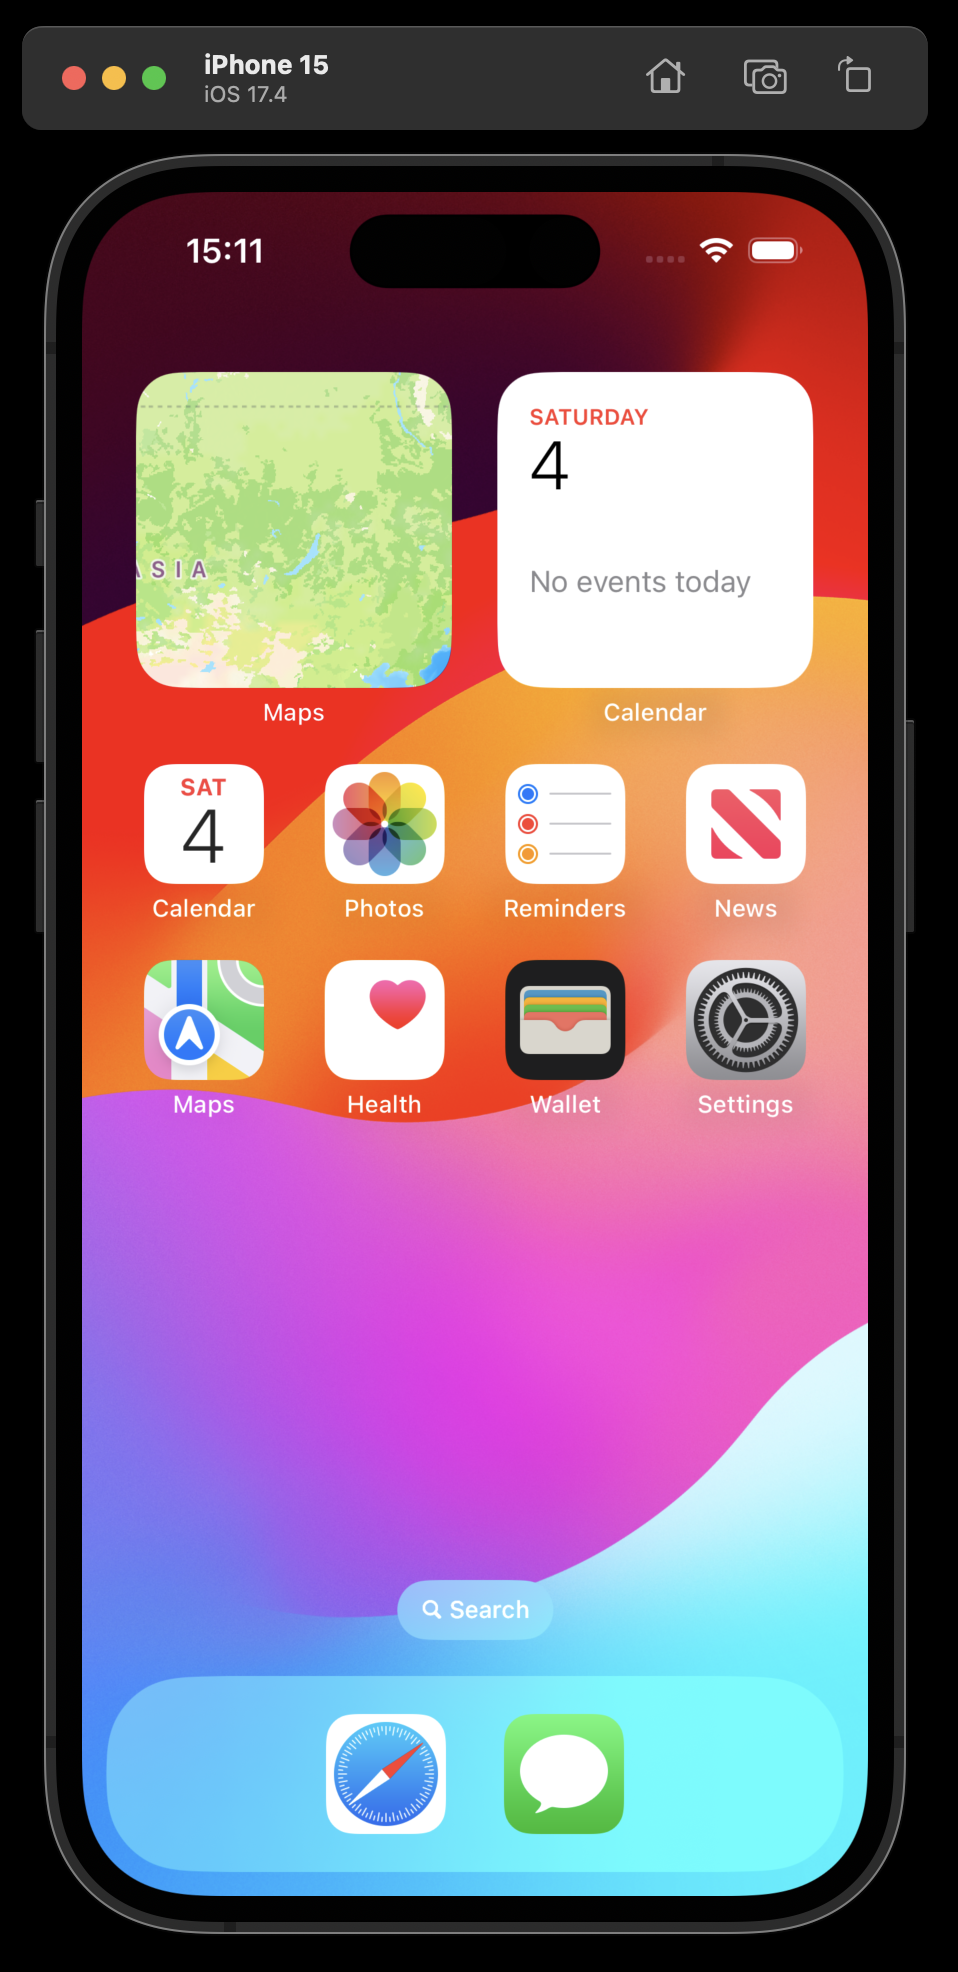
\includegraphics[width=0.25\textwidth]{images/task-1/1.png}
  \caption{Эмулятор iOS}
  \label{fig:task-1-1}
\end{figure}

Затем, перейдя в одноименную директорию <<\foreignlanguage{english}{my\_app}>>,
была выполнена команда <<\foreignlanguage{english}{flutter run}>>. После
выполнения данной команды приложение было открыто в эмуляторе iOS (рисунок
\ref{fig:task-1-2}).

\begin{figure}[H]
  \centering
  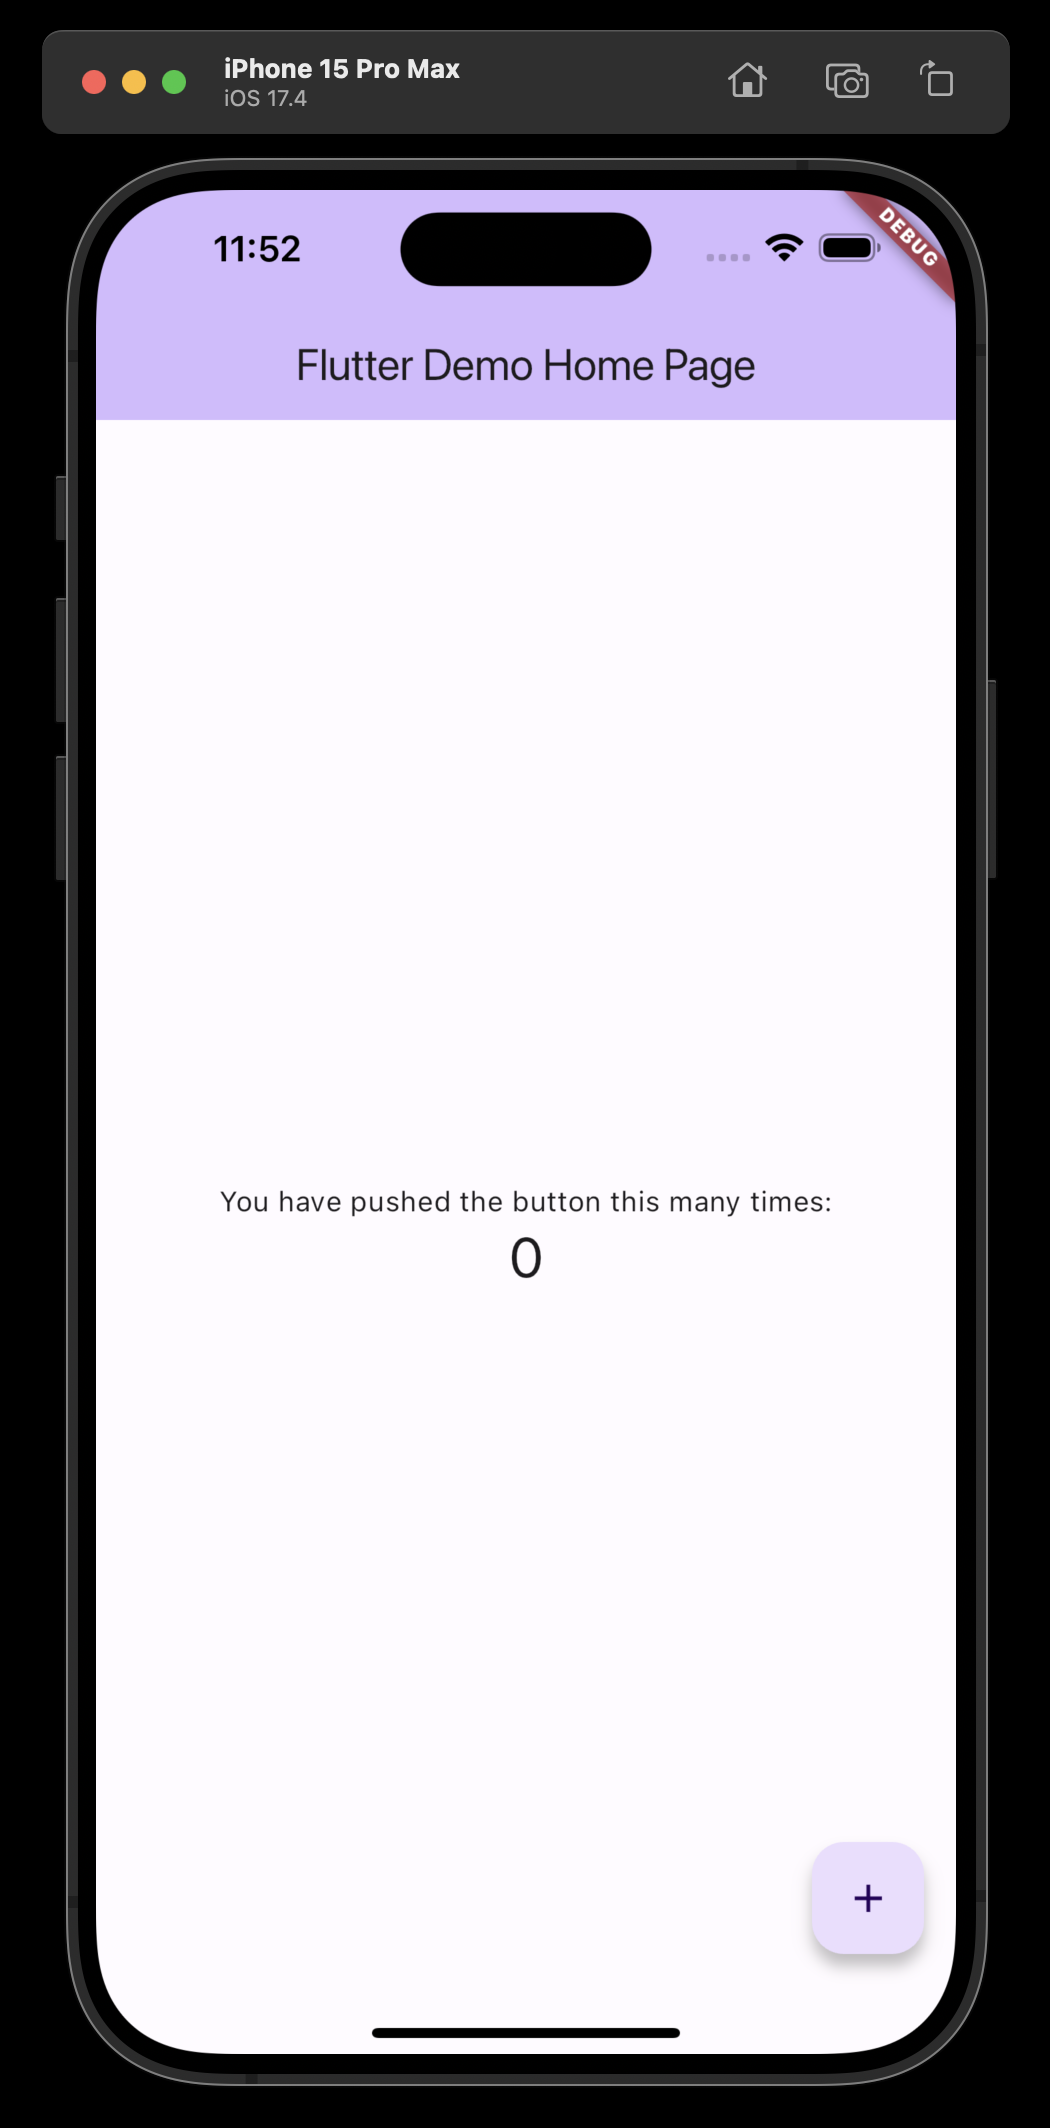
\includegraphics[width=0.25\textwidth]{images/task-1/2.png}
  \caption{Запущенное приложение в эмуляторе iOS}
  \label{fig:task-1-2}
\end{figure}

После этого исходный код созданного приложения был изменен в соответствии с
примером из видео-уроков. После запуска получившейся программы, открылось
приложение, показанное на рисунке \ref{fig:task-1-3}.

\begin{figure}[H]
  \centering
  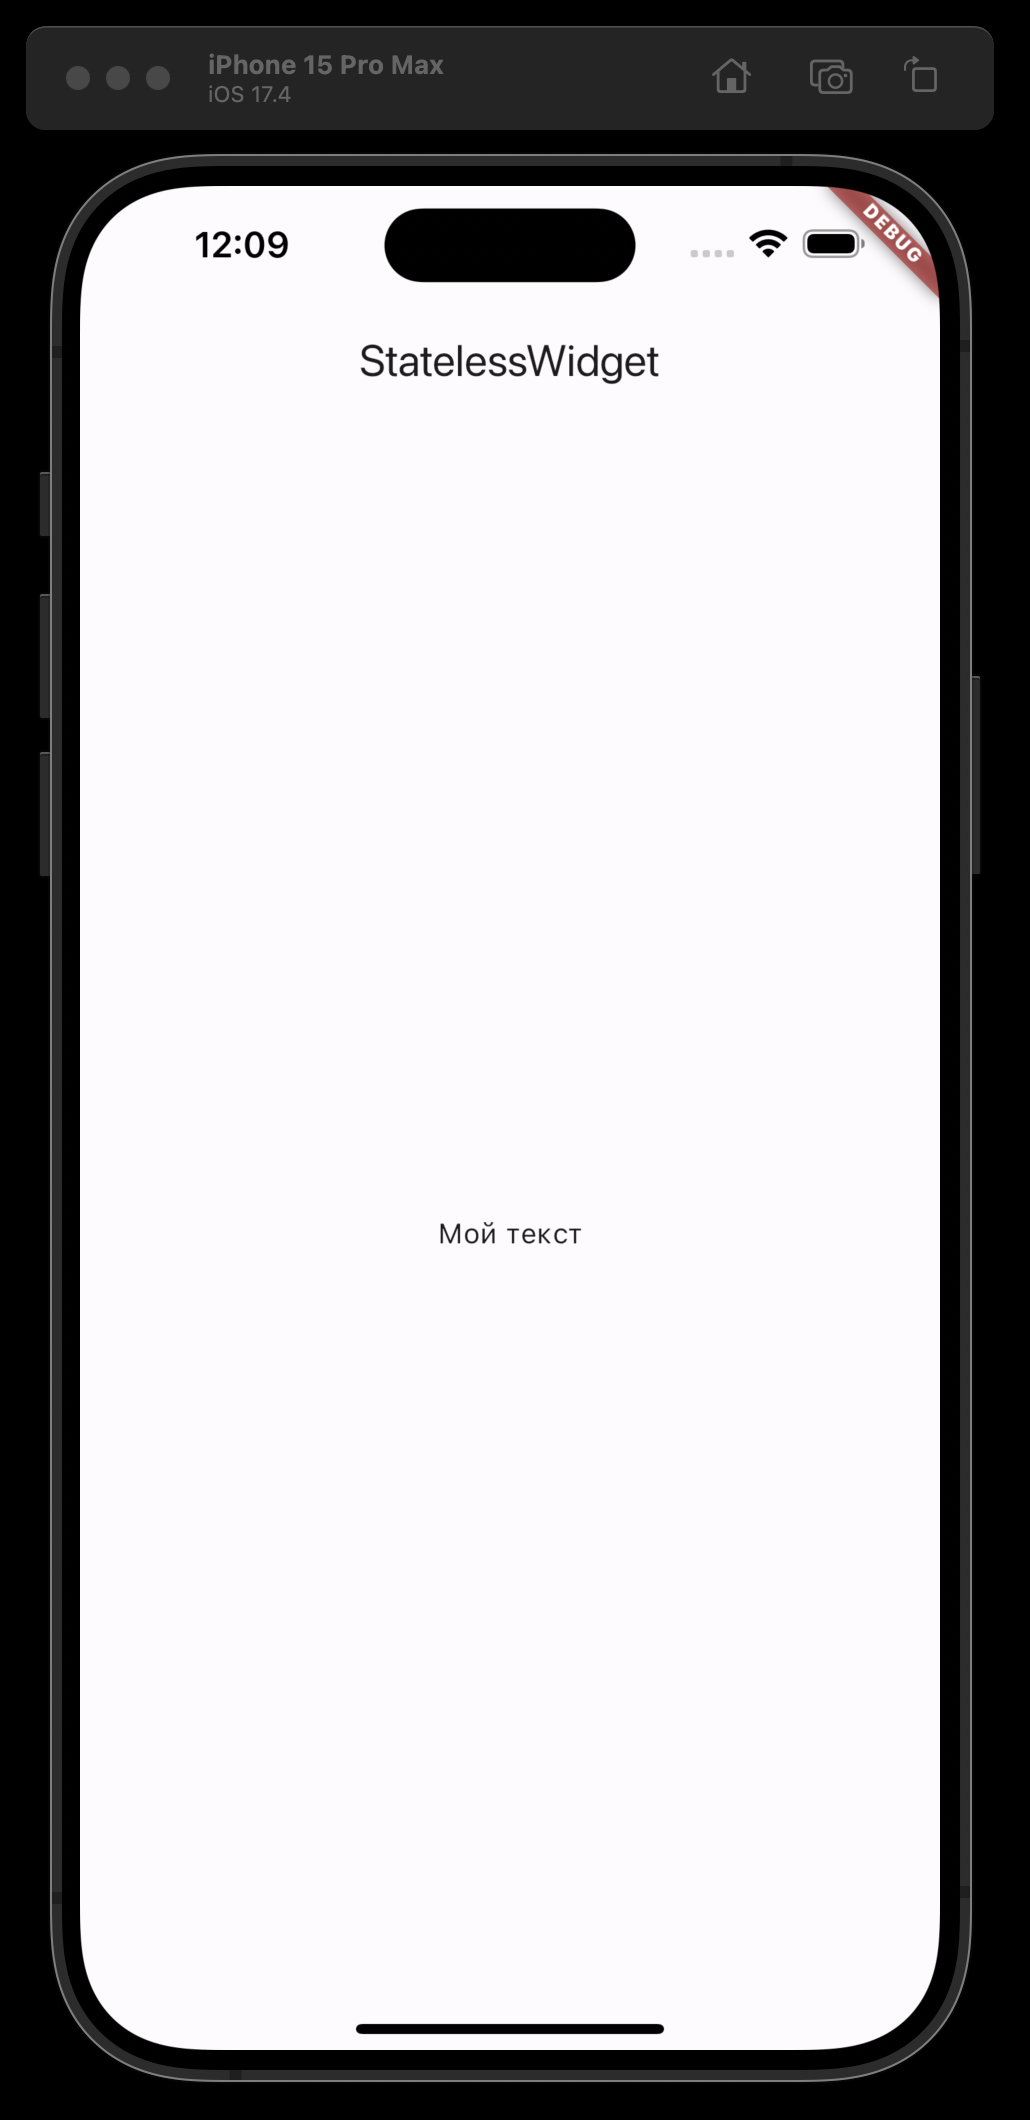
\includegraphics[width=0.25\textwidth]{images/task-1/3.png}
  \caption{Запущенное приложение в эмуляторе iOS}
  \label{fig:task-1-3}
\end{figure}

\subsection*{Создание мобильного клиента PostgreSQL}

После этого было разработан мобильный клиент PostgreSQL, который позволяет
выполнять запросы и получать вывод в виде таблиц. На рисунке \ref{fig:task-2-1}
экран, который приветствует пользователя. В нем пользователю необходимо ввести
адрес и порт СУБД, а также имя пользователя и пароль.

\begin{figure}[H]
  \centering
  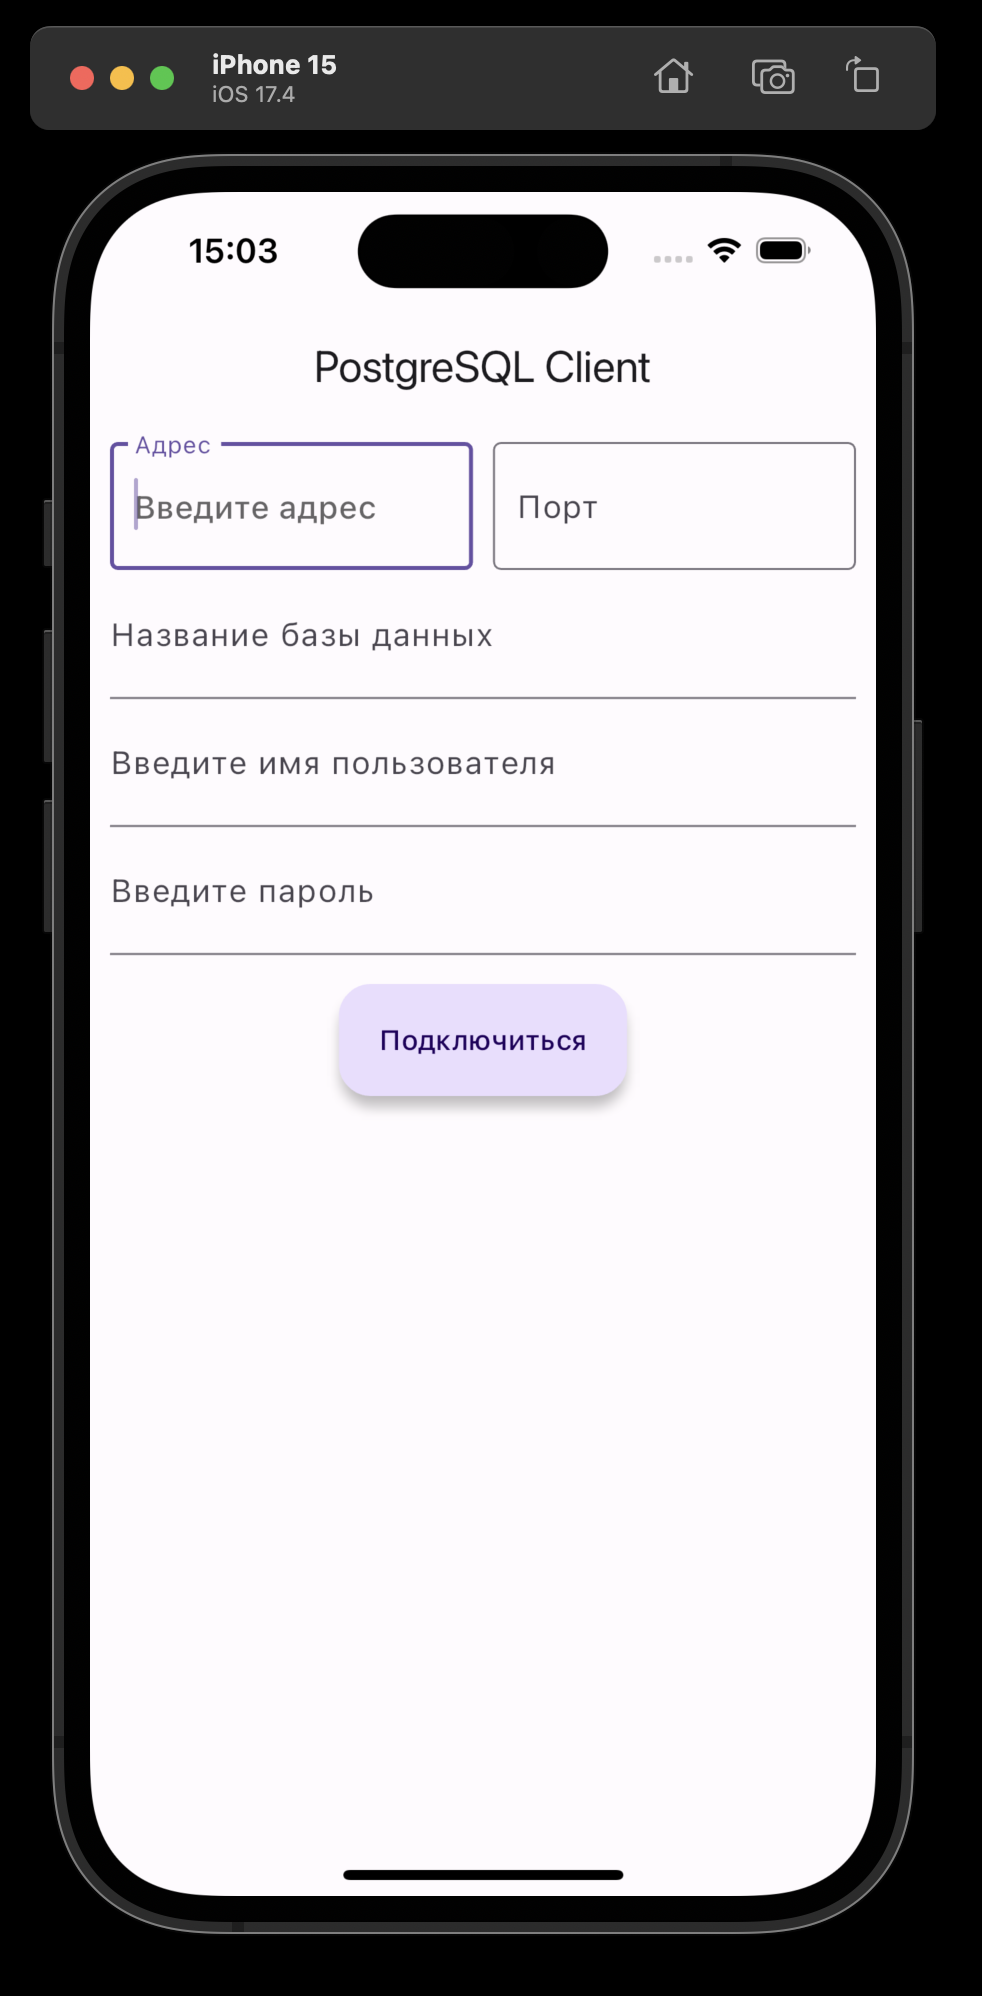
\includegraphics[width=0.25\textwidth]{images/task-2/1.png}
  \caption{Экран, отображаемый при открытии приложения}
  \label{fig:task-2-1}
\end{figure}

После ввода данных, например, как показано на рисунке \ref{fig:task-2-2},
пользователю необходимо нажать на кнопку <<Подключиться>>. После нажатия на эту
кнопку будет установлено соединение с базой данных. Если соединение было
установлено успешно, пользователя перекинет на экран, показанный на рисунке
\ref{fig:task-2-3}. В нем пользователю предлагается вводить и выполнять запросы.

\begin{figure}[H]
  \centering
  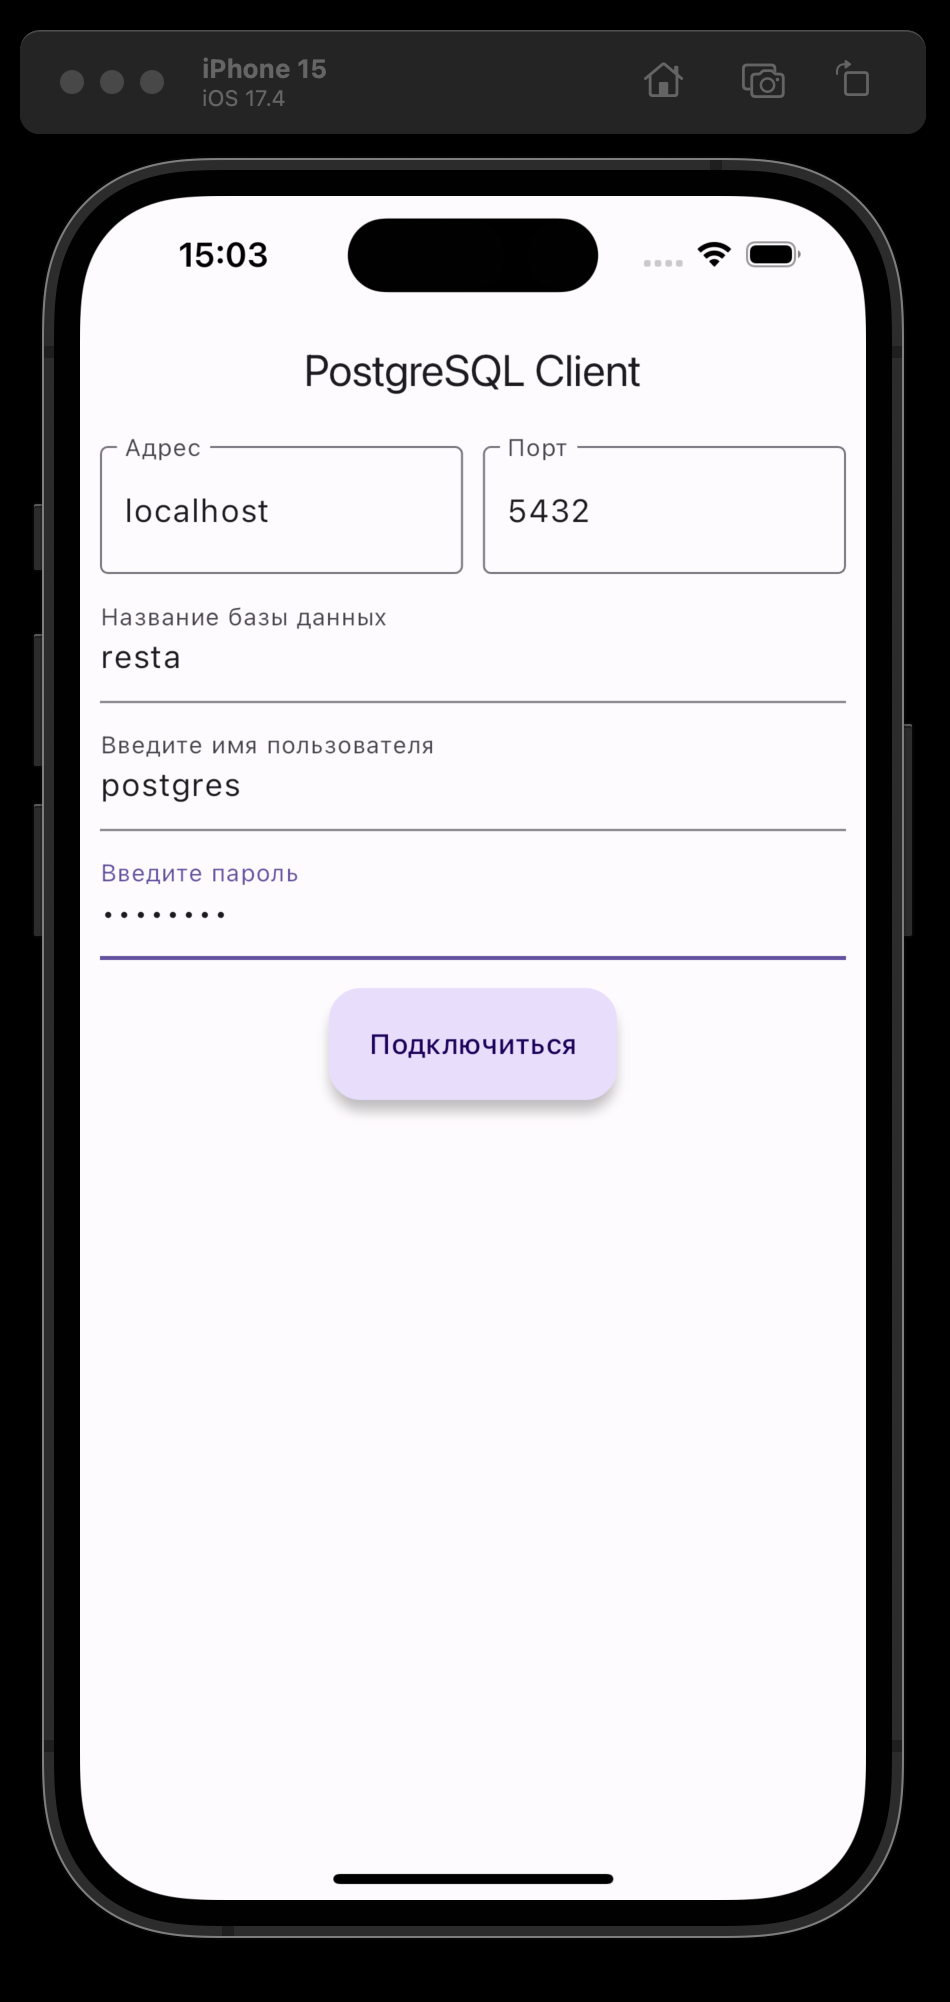
\includegraphics[width=0.25\textwidth]{images/task-2/2.png}
  \caption{Пример ввода данных СУБД}
  \label{fig:task-2-2}
\end{figure}

\begin{figure}[H]
  \centering
  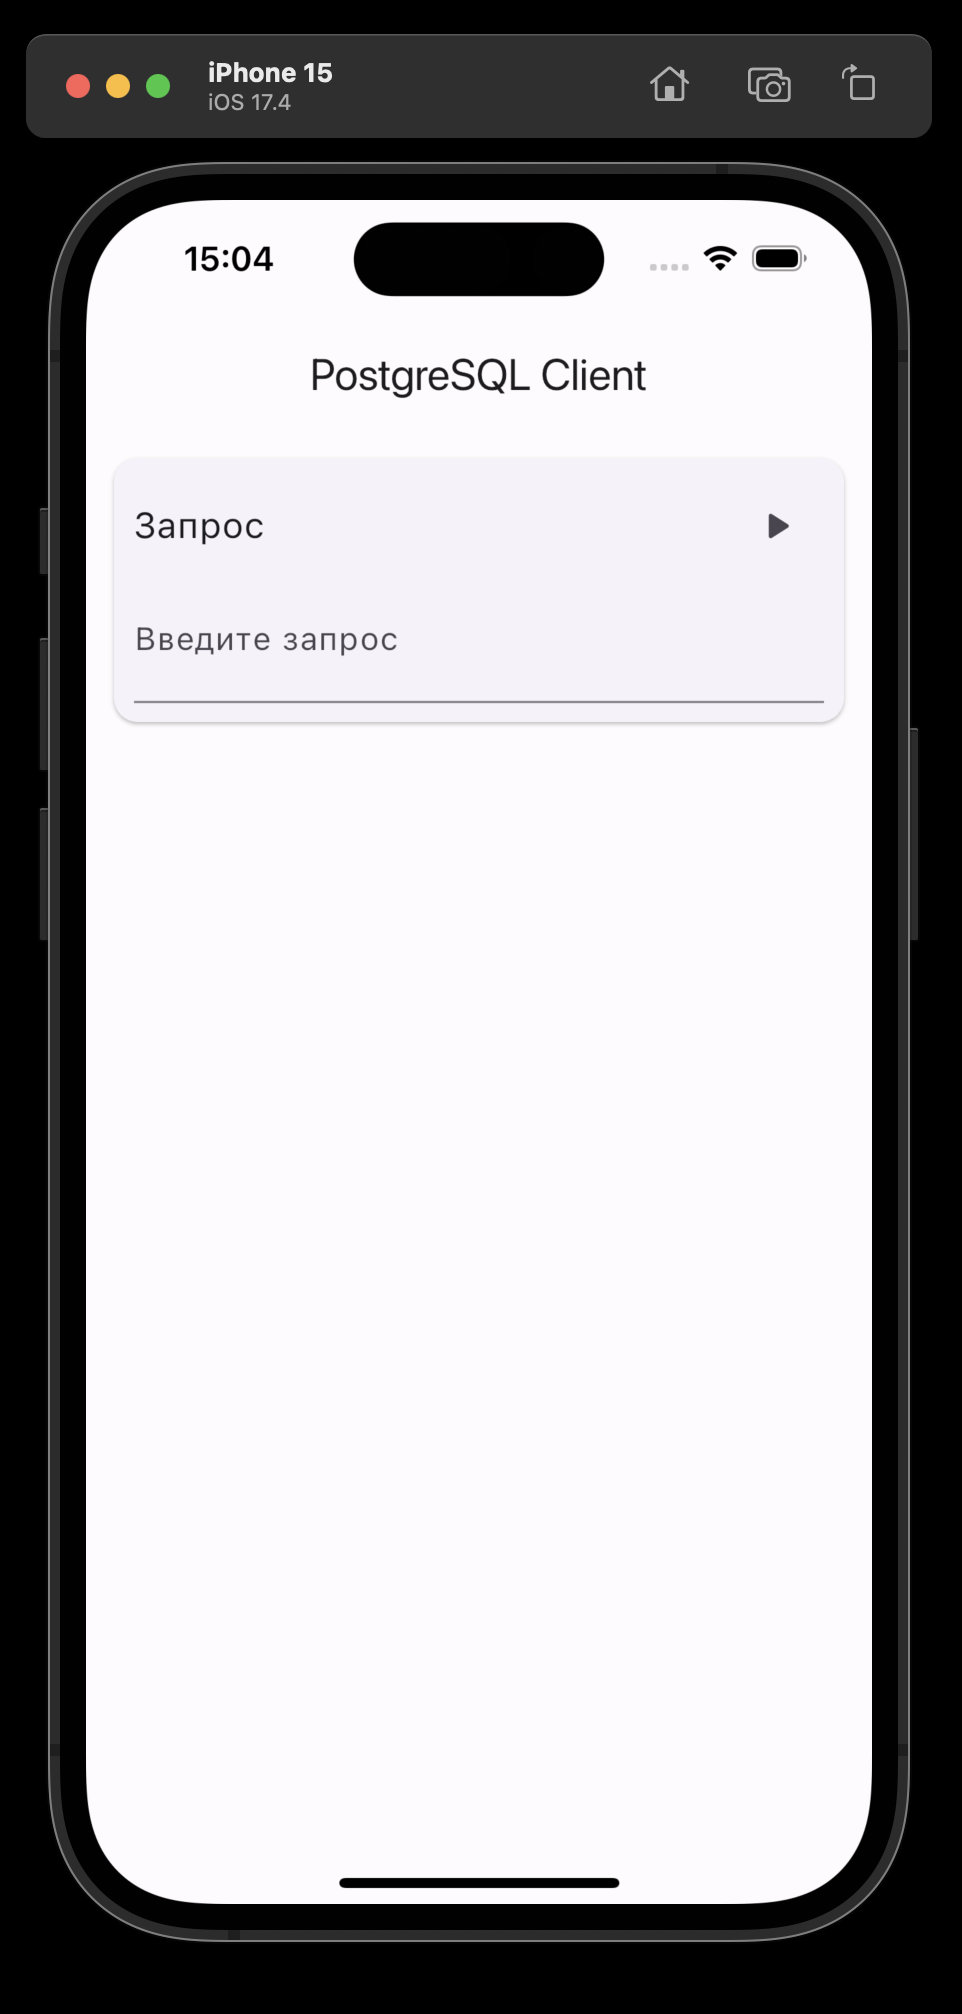
\includegraphics[width=0.25\textwidth]{images/task-2/3.png}
  \caption{Экран для выполнения запросов}
  \label{fig:task-2-3}
\end{figure}

На рисунке \ref{fig:task-2-4} приведен пример выполнения запроса. В текстовое
поле был введен запрос, содержащий оператор
<<\foreignlanguage{english}{SELECT}>>, после чего была нажата кнопка выполнения
запроса. После этого на экране пользователя появилась таблица, которая содержит
данные из СУБД.

\begin{figure}[H]
  \centering
  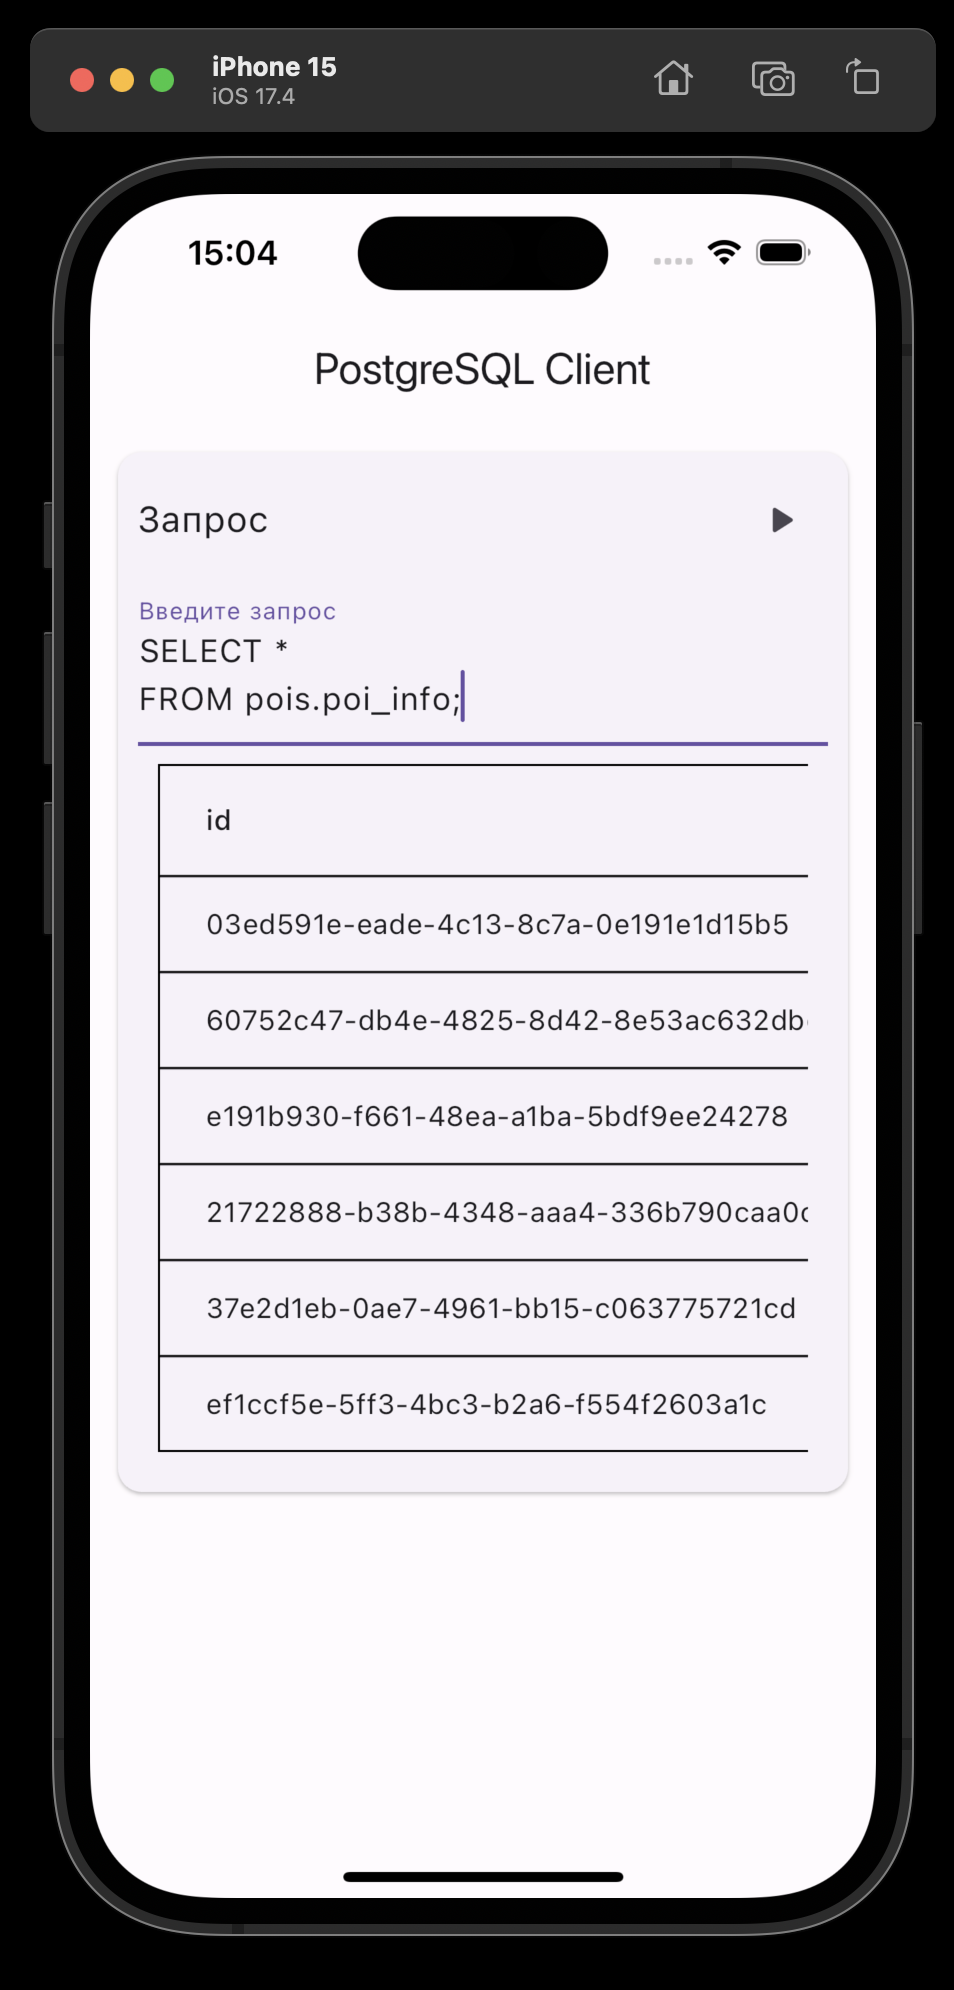
\includegraphics[width=0.25\textwidth]{images/task-2/4.png}
  \caption{Пример выполнения запроса}
  \label{fig:task-2-4}
\end{figure}

\section{Вывод}

В данной лабораторной работе было разработано мобильное приложение для
подключения к БД \foreignlanguage{english}{PostgreSQL} с помощью
\foreignlanguage{english}{Flutter}. Цель, поставленная в начале работы,
достигнута, задачи выполнены.

\end{document}
